%
% dimension.tex
%
% (c) 2021 Prof Dr Andreas Müller, OST Ostschweizer Fachhochschule
%
\bgroup
\definecolor{darkgreen}{rgb}{0,0.6,0}
\begin{frame}[t]
\frametitle{Dimension von $\mathcal{K}^k(f)$ und $\mathcal{J}^k(f)$}
\begin{center}
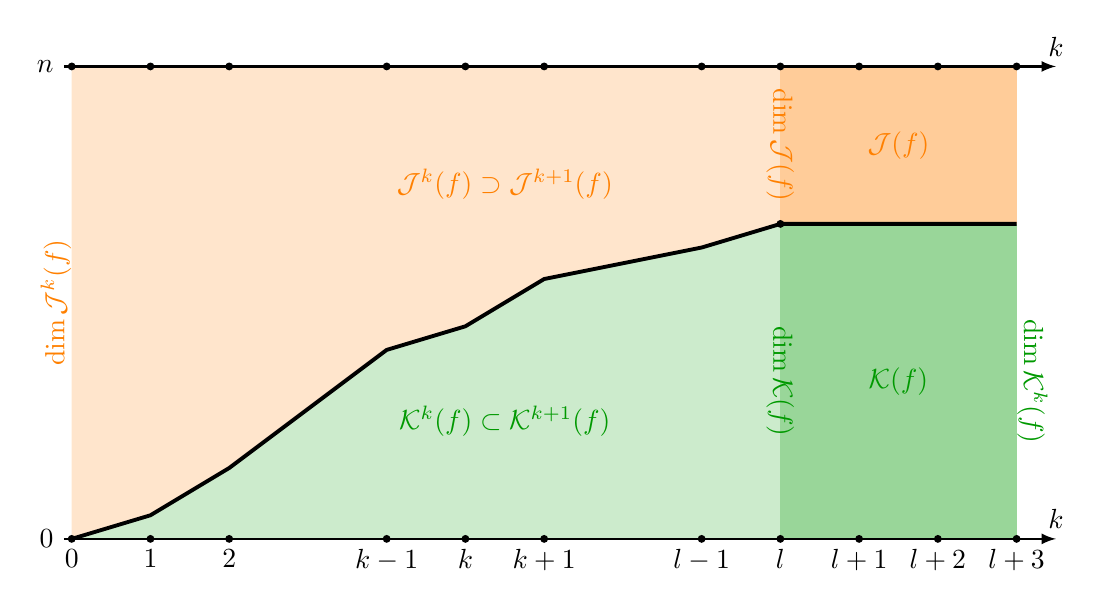
\begin{tikzpicture}[>=latex,thick]

\def\pfad{
	(0,0) -- (1,0.3) -- (2,0.9) 
	--
	(4,2.4) -- (5,2.7) -- (6,3.3)
	--
	(8,3.7) -- (9,4) -- (10,4) -- (11,4) -- (12,4)
}

\fill[color=darkgreen!20] \pfad -- (12,0) -- cycle;
\fill[color=orange!20] \pfad -- (12,6) -- (0,6) -- cycle;

\fill[color=darkgreen!40] (9,0) -- (12,0) -- (12,4) -- (9,4) -- cycle;
\fill[color=orange!40] (9,4) -- (12,4) -- (12,6) -- (9,6) -- cycle;

\node[color=orange] at (10.5,5) {$\mathcal{J}(f)$};
\node[color=darkgreen] at (10.5,2) {$\mathcal{K}(f)$};

\node[color=orange] at (5.5,4.5) {$\mathcal{J}^k(f)\supset\mathcal{J}^{k+1}(f)$};
\node[color=darkgreen] at (5.5,1.5) {$\mathcal{K}^k(f)\subset\mathcal{K}^{k+1}(f)$};

\draw[line width=1.4pt] \pfad;

\draw[->] (-0.1,6) -- (12.5,6) coordinate[label={$k$}];
\draw[->] (-0.1,0) -- (12.5,0) coordinate[label={$k$}];
\node at (-0.1,6) [left] {$n$};
\node at (-0.1,0) [left] {$0$};
\foreach \x in {0,1,2,4,5,6,8,9,10,11,12}{
	\fill (\x,0) circle[radius=0.05];
	\fill (\x,6) circle[radius=0.05];
}
\node at (0,0) [below] {$0$};
\node at (1,0) [below] {$1$};
\node at (2,0) [below] {$2$};

\node at (4,0) [below] {$k-1$};
\node at (5,0) [below] {$k$};
\node at (6,0) [below] {$k+1$};

\node at (8,0) [below] {$l-1$};
\node at (9,0) [below] {$l$};
\node at (10,0) [below] {$l+1$};
\node at (11,0) [below] {$l+2$};
\node at (12,0) [below] {$l+3$};

\fill (9,4) circle[radius=0.05];

\node[color=orange] at (-0.2,3) [rotate=90] {$\dim\mathcal{J}^k(f)$};
\node[color=darkgreen] at (12.2,2) [rotate=-90] {$\dim\mathcal{K}^k(f)$};

\node[color=orange] at (9,5) [rotate=-90] {$\dim\mathcal{J}(f)$};
\node[color=darkgreen] at (9,2) [rotate=-90] {$\dim\mathcal{K}(f)$};

\end{tikzpicture}
\end{center}

\end{frame}
